\section{Mise en place d'une solution \acentreon{}}

\subsection{La solution \acentreon}

\paragraph{}
\acentreon{} est une plateforme open source de supervision, c'est-à-dire de surveillance du bon fonctionnement d'une infrastructure système.

\paragraph{Principe de la supervision}
De façon classique, on surveille toutes les informations relatives au matériel (température, pannes\ldots) et au système (charge serveur, utilisation de la mémoire et du processeur\ldots) des serveurs d'un parc.
Généralement, on supervise également tous les services applicatifs (serveurs web, serveurs FTP, serveurs de base de données\ldots) qui y sont hébergées.

Ainsi, les administrateurs système peuvent savoir en temps réel quels sont les services et les machines qui sont fonctionnels ou hors-service.
Très souvent, des alertes leurs sont envoyées pour les prévenir d'une rupture de service.
Ces alertes peuvent prendre la forme d'e-mails mais aussi de SMS ou de messages envoyés par messagerie instantanée.

\paragraph{\anagios}
La solution \acentreon{} repose sur \anagios{} pour effectuer toutes les opérations de surveillance, de reporting et de d'alerte.
Par défaut, \anagios{} propose un certain nombre de possibilités que ce soit pour superviser les ressources des serveurs, les services actifs en consultant un port\footnote{Correspondant à la couche de transport du modèle OSI, la notion de port logiciel permet, sur un ordinateur donné, de distinguer différents interlocuteurs. Ces interlocuteurs sont des programmes informatiques qui, selon les cas, écoutent ou émettent des informations sur ces ports. Un port est distingué par son numéro.~\cite{port}} donné ou en interrogeant les machines via le protocole SNMP\footnote{SNMP (pour \etranger{Simple Network Management Protocol}) est un protocole de communication qui permet aux administrateurs réseau de gérer les équipements du réseau, de superviser et de diagnostiquer des problèmes réseaux et matériels à distance.~\cite{snmp}}.

Les possibilités de supervision sont infinies car \anagios{} est doté d'un système de plugins très efficace.
En effet, ces plugins sont de simples programmes exécutables via la ligne de commande, auxquels on passe en paramètre des options de configuration et qui retournent un entier.
On peut donc les développer dans n'importe quel langage de programmation.
C'est la valeur du code retour qui précise si le test effectué par le plugin est passé ou non :

\begin{description}
	\item[0 OK] le test est passé ;
	\item[1 WARNING] le seuil d'alerte est dépassé ;
	\item[2 CRITICAL] le service a un problème ;
	\item[3 UNKNOWN] il est impossible de connaître l'état du service.
\end{description}

Ces différents niveaux, en plus de permettre le déclenchement d'alertes, sont facilement distinguables sur l'interface web de \anagios{} via un code couleur (\cffigure{centreon:nagios}).

Enfin, il est possible de lancer des actions de surveillance à distance via le protocole NRPE (\etranger{Nagios Remote Plugin Executor}).
En effet, celui-ci permet de lancer n'importe quel plugin \anagios{}, si celui-ci est bien installé sur la machine interrogée.
Les informations transitent entre le serveur \anagios{} et les machines surveillées via un tunnel SSL\footnote{SSL (pour \etranger{Secure Sockets Layer}) est un protocole de sécurisation des échanges sur Internet.~\cite{tls}} sécurisé.

\begin{figure}
	\centering
	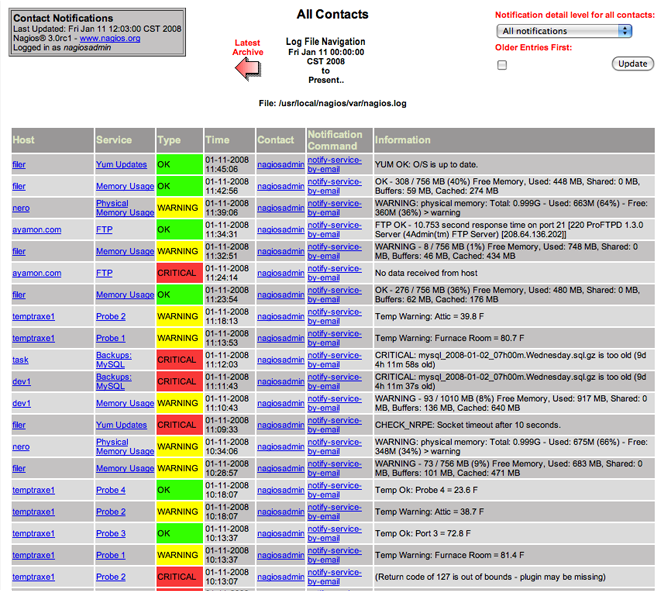
\includegraphics[width=12cm]{centreon/nagios-notifications}
	\caption{Historique des notifications sur Nagios}
	\label{figure:centreon:nagios}
\end{figure}

\paragraph{\acentreon}
Le principal avantage de ce complément à \anagios{} est de fournir une interface graphique web efficace, claire et plus simple à appréhender (\cffigure{centreon:centreon}).

Il ajoute entre autres une gestion fine des utilisateurs, des plugins \anagios{} supplémentaires, des représentations graphiques élaborées, des possibilités d'architecture distribuée, etc.

\begin{figure}
	\centering
	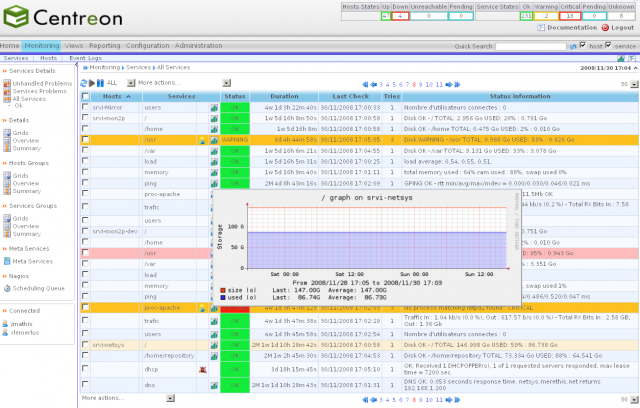
\includegraphics[width=12cm]{centreon/centreon-status}
	\caption{État en temps réel des services sur \acentreon{}}
	\label{figure:centreon:centreon}
\end{figure}


\subsection{Contexte de la mission}


\subsection{Notre démarche}

location serveur
install centreon

configuration des pluugins




